\section{Introduction}

\subsection{Electricity Market Modeling}

\begin{frame}					
\frametitle{Electricity Market Modeling}

\begin{figure}[h]
\centering
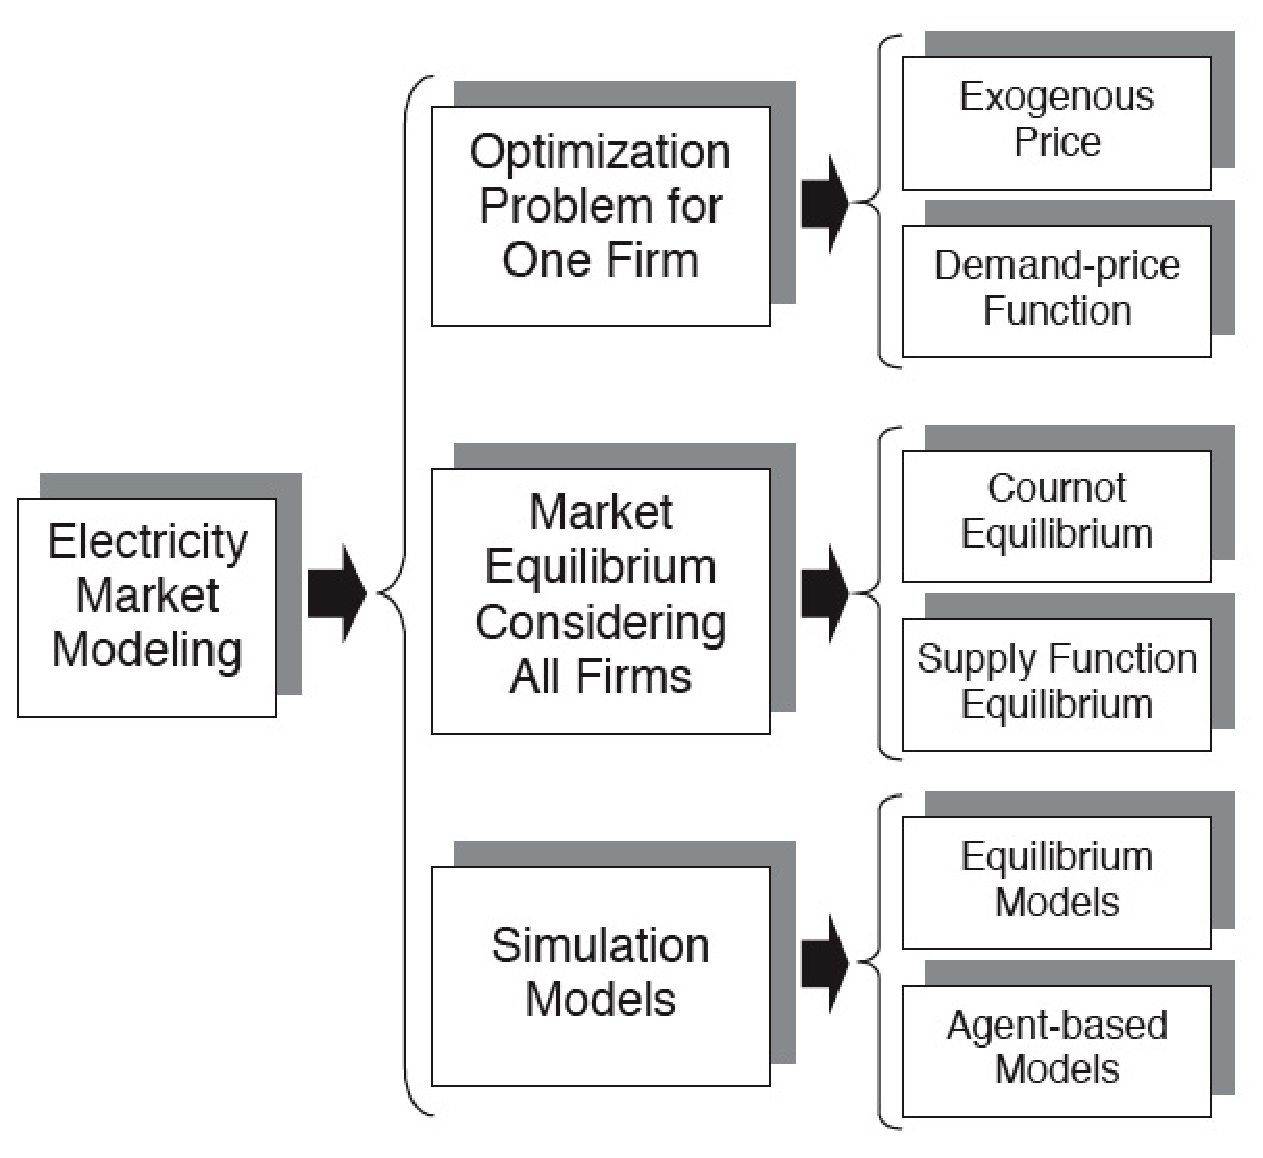
\includegraphics[width=0.7\textwidth]{introduction/ventosa1.pdf}
    \caption{Ventosa et. al (2005)}
    \label{fig:ventosa1}            
\end{figure}
\end{frame}

\subsection{Mathematical Structure of Optimization Problem}

\begin{frame}
\frametitle{Mathematical Structure of Optimization Problem}
%\begin{columns}
%\begin{column} {0.6\textwidth}
\begin{figure}[h]
\centering
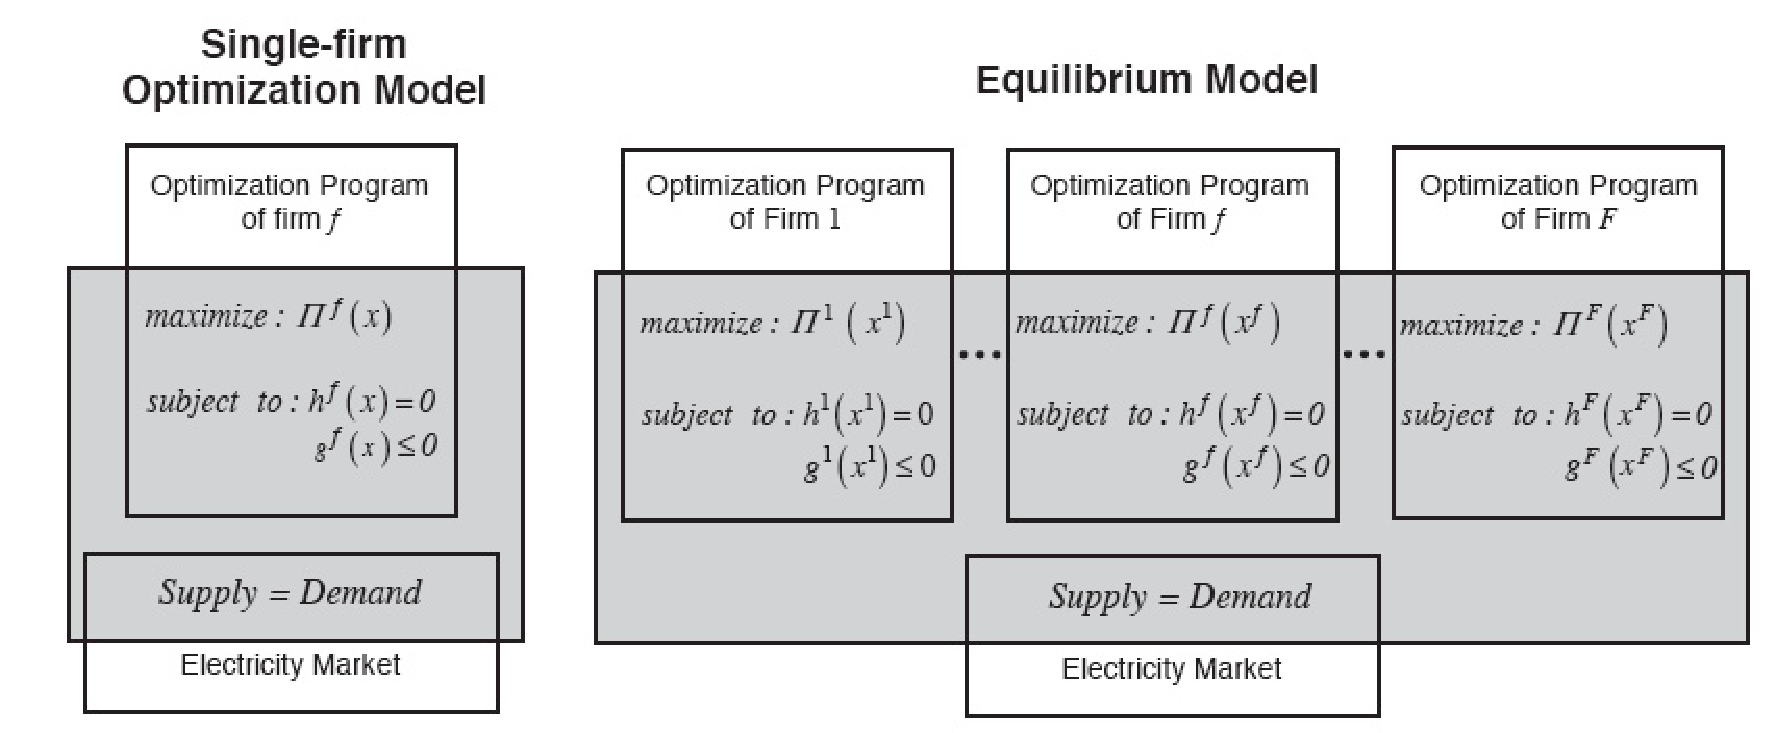
\includegraphics[width=1.\textwidth]{introduction/ventosa2.pdf}
    \caption{Ventosa et. al (2005)}
    \label{fig:ventosa2}            
\end{figure}
%\end{column}
%\begin{column} {0.4\textwidth}
%\begin{itemize}
%	\item bla
%\end{itemize}	
%\end{column}
%\end{columns}
\end{frame}

\subsection{Investment Decision Models}

\begin{frame}
\frametitle{Investment Decision Models}
\begin{itemize}
         \item \textcolor{craneblue}{\textbf{Expansion planning game:}} Chuang et al. (2001)\\
         \begin{itemize}
         		\item new plant construction at single point in time with multiple technology options
		\item monopoly may lack sufficient incentives to introduce new technologies
	\end{itemize}         
                  \item \textcolor{craneblue}{\textbf{Comparison of two approaches for expansion planning:}} Ventosa et al. (2002)\\
         \begin{itemize}
         		\item Firms decide output and generating capacity in a Cournot manner\\ 
		$\Rightarrow$ \emph{Mixed Linear Complementarity Problem (LCP)}
		\item Leader firm that anticipates reaction of follower firm as Stackelberg game\\
		$\Rightarrow$ \emph{Mathematical Program with Equilibrium Constraints (MPEC)}
	\end{itemize}  
         \item \textcolor{craneblue}{\textbf{Stochastic demand growth:}} Pineau and Murto (2003)\\
         \begin{itemize}
         		\item $S$-adapted open-loop information structure
	\end{itemize}
	\item \textcolor{craneblue}{\textbf{Stochastic programming formulation:}} Genc et al. (2007)
         \begin{itemize}
         		\item games with probabilistic scenarios (GPS)
		\item  $S$-adapted open-loop information structure
	\end{itemize}	
	\item \textcolor{craneblue}{\textbf{Cross-price effects:}} Pineau and Zaccour (2007)
         \begin{itemize}
         		\item increased cross-price elasticity leads to overall decrease of total capacity
	\end{itemize}	
\end{itemize}

\end{frame}